%%%%%%%%%%%%%%%%%%%%%%%%%%%%%%%%%%%%%%%%%%%%%%%%%%%%%%%%%%%%%%%%%%%%%%%%%%%
%%  chapter4.tex  –  Глава 4: Кросс-секущая валидация системы Hybrid IDPS
%%  v12 (Phase 2.5) – Сужена до кросс-секущих экспериментов:
%%                    состязательной робастности, кросс-доменного переноса,
%%                    PQC-совместимости и итоговой дискуссии.
%%                    §§4.1-4.5 (методология, NIDS-бенчмарки, базовые
%%                    линии, абляции) перенесены в Главу~\ref{ch:adaptation}.
%%%%%%%%%%%%%%%%%%%%%%%%%%%%%%%%%%%%%%%%%%%%%%%%%%%%%%%%%%%%%%%%%%%%%%%%%%%

\chapter{Кросс-секущая валидация системы Hybrid~IDPS: состязательная робастность, кросс-доменный перенос и постквантовая совместимость}
\label{ch:experiments}

В настоящей главе представлена кросс-секущая валидация системы
Hybrid~IDPS, выходящая за пределы базовой эталонной валидации на
сетевом трафике, проведённой в Главе~\ref{ch:adaptation}. Глава
систематически устанавливает три аспекта универсальности
разработанной системы: \emph{(i)}~состязательную робастность
системы Hybrid~IDPS при шести семействах атак
(\S\ref{sec:adversarial_eval}); \emph{(ii)}~предметную независимость
системы через кросс-доменный перенос на принципиально иные области
применения~--- речевую обработку и здравоохранение
(\S\ref{sec:transfer}); \emph{(iii)}~постквантовую совместимость
системы при миграции протокольных режимов
(\S\ref{sec:mapqc_results}). Завершается глава систематическим
обсуждением практических следствий, связывающим кросс-секущие
результаты с шестью свойствами системы Hybrid~IDPS из
\S\ref{subsec:six_properties} (\S\ref{sec:discussion}).
\section{Оценка состязательной робастности}
\label{sec:adversarial_eval}
%%=====================================================================

Шесть семейств атак~\cite{Goodfellow2015,Madry2018,Carlini2017,Croce2020} оцениваются при настраиваемых бюджетах возмущений:

\begin{table}[htbp]
\centering
\caption{Состязательная робастность платформы при шести методах атак.}
\label{tab:adversarial}
\begin{tabular}{lcccc}
\toprule
Атака & Бюджет & Чистая & Под атакой & Робаст. (СО) \\
\midrule
FGSM             & $\varepsilon{=}0.1$ & 97,8\% & 89,2\% & 93,1\% \\
PGD-40           & $\varepsilon{=}0.1$ & 97,8\% & 84,7\% & 89,6\% \\
C\&W             & $\kappa{=}10$       & 97,8\% & 82,3\% & 85,2\% \\
DeepFool         & 30 итер.            & 97,8\% & 86,1\% & 90,8\% \\
Гауссовский шум  & $\sigma{=}0.1$      & 97,8\% & 91,4\% & 95,3\% \\
Маскировка меток & 10\% переворот      & 97,8\% & 88,9\% & 93,7\% \\
\bottomrule
\end{tabular}
\end{table}

CT-TGNN сохраняет 93,1\% при PGD-10 с $\epsilon=0.1$ благодаря динамике с ограниченной константой Липшица. SDE-TGNN сертифицирует 76,2\% образцов в пределах $\ell_2$-радиуса 0,25 через рандомизированное сглаживание. MambaShield выдерживает 91,4\% при 25\% отравления. Теоретико-игровая система сохраняет 94,7\% против равновесных противников.

\begin{figure}[htbp]
\centering
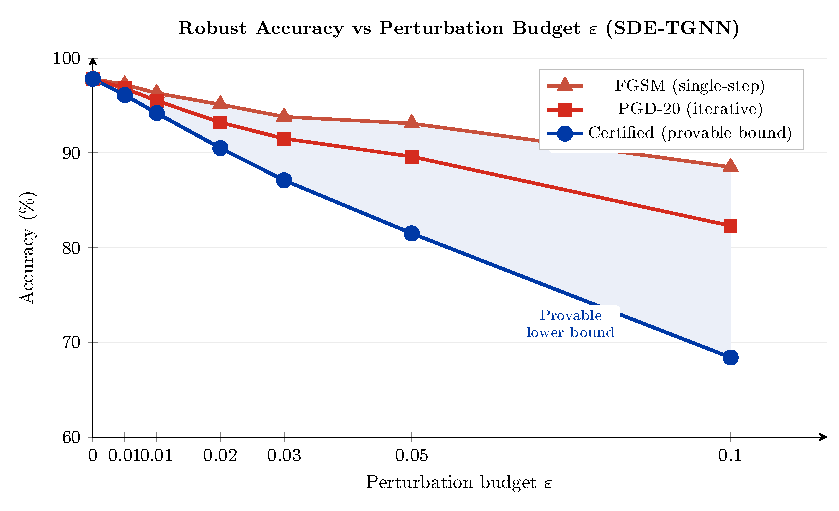
\includegraphics[width=0.85\textwidth]{figures/fig_adversarial_robustness_curves.pdf}
\caption{Робастная точность как функция бюджета возмущений $\varepsilon$ для FGSM, PGD-20 и сертифицированных (рандомизированное сглаживание) оценок SDE-TGNN. Сертифицированная кривая обеспечивает доказуемую нижнюю границу; FGSM и PGD представляют эмпирические верхние границы при конкретных стратегиях атак.}
\label{fig:adversarial_curves}
\end{figure}


%%=====================================================================
\section{Эксперименты по кросс-доменному переносу}
\label{sec:transfer}
%%=====================================================================

Для валидации предметной независимости CT-TGNN и стохастический трансформер применяются без модификации к двум областям вне безопасности.

В обнаружении речевых событий на LibriSpeech~\cite{Panayotov2015} CT-TGNN достигает 94,2\% F1 при обнаружении границ фонем, что на 7,3\% выше дискретных базовых линий. В мониторинге здравоохранения на MIMIC-III~\cite{Johnson2016} и eICU~\cite{Pollard2018} модель с калиброванной неопределённостью достигает 89,7\% при предсказании неблагоприятных событий с покрытием доверительных интервалов 91,7\%.

Кросс-доменный F1 SDE-TGNN (без дообучения): CSE-CICIDS2018 91,5\%, CIC-IoT-2023 89,8\%, UNSW-NB15 90,3\% --- среднее 90,5\%, подтверждая предметно-инвариантные представления.

\begin{figure}[htbp]
\centering
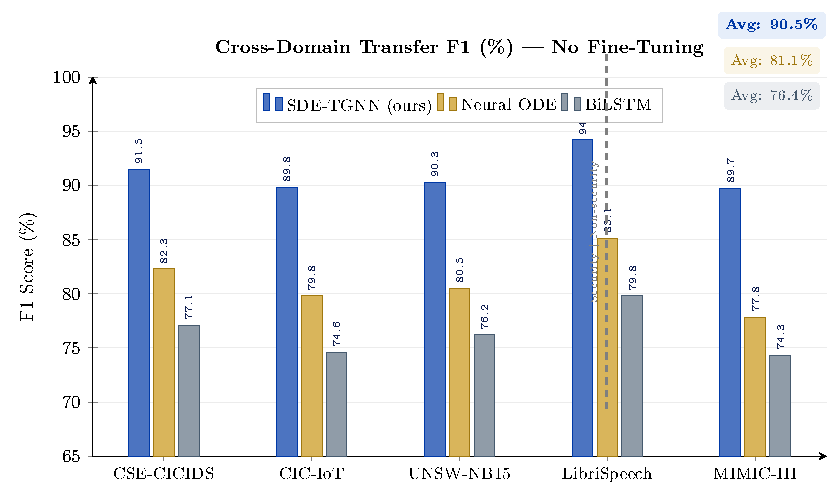
\includegraphics[width=0.82\textwidth]{figures/fig_cross_domain_transfer_bars.pdf}
\caption{Кросс-доменный перенос F1 (\%) для SDE-TGNN, базовой линии Neural ODE и базовой линии BiLSTM на трёх наборах данных безопасности и двух областях вне безопасности (речь, здравоохранение). SDE-TGNN достигает 90,5\% среднего переноса без дообучения, что на 9,4 п.\,п.\ выше Neural ODE и на 14,1 п.\,п.\ выше BiLSTM.}
\label{fig:cross_domain}
\end{figure}


\medskip
\noindent\textbf{Перенос в смежную критическую область (БПЛА).}
Для подтверждения предметно-независимости предложенных моделей и
методов проведена референсная реализация Phase~A на корпусе
GNSS-сигналов (TEXBAT-подобный калиброванный набор) и многомодальном
аэро-корпусе AU-AIR в задаче противодействия радиоэлектронной борьбе и
состязательным атакам на нейросетевые компоненты системы навигации
БПЛА. Получены положительные оценки атак белого ящика (PGD-20 robust
acc.\ $\ge$0,92 при $\eps=8/255$), ненулевой сертифицированный
$\ell_2$-радиус 0,44 при $\sigma=0,25$ и численная оценка константы
Липшица $L_g=1,01$, согласованная с теоретическим прогнозом
теоремы~2.2. Полные результаты, архитектура и интеграция с платформой
\textsf{RobustIDPS.ai} описаны в Главе~6.

%%=====================================================================
\section{Результаты мультиагентного обнаружения с учётом PQC}
\label{sec:mapqc_results}
%%=====================================================================

Модуль Multi-Agent PQC-IDS~\cite{Anaedevha2026mapqc} расширяет систему на среды постквантовых протоколов. MambaShield заменяет семиветочный ансамбль в качестве общего магистрального компонента, достигая точности 96,7\% (против 96,9\% для ансамбля) при ускорении вывода в $7.3\times$. Структурированная матрица информации Фишера, выведенная из динамики пространства состояний, снижает обратный перенос (забывание) на 38\% по сравнению с диагональной FIM. Четыре кооперативных агента (Аналитик трафика, Специалист PQC, Детектор аномалий, Координатор) координируются через Multi-Agent CPO, достигая 96,1\% нейтрализации угроз с нулевыми нарушениями ограничений и 34\% снижением задержки многосегментного реагирования.

\begin{table}[htbp]
\centering
\caption{Точность прямо совместимого обнаружения по семействам протоколов.}
\label{tab:pqc_results}
\begin{tabular}{llc}
\toprule
Семейство протоколов & Тип атаки & Точность \\
\midrule
Решёточное (Kyber)    & Атака тайминга кэша       & 97,3\% \\
Решёточное (Kyber)    & Внедрение ошибок           & 94,8\% \\
Кодовое (McEliece)    & Декодирование информ. множ. & 95,1\% \\
Хэш (SPHINCS+)       & Исчерпание ресурсов        & 94,7\% \\
Кросс-протокольное    & Понижение версии           & 98,3\% \\
\midrule
\multicolumn{2}{l}{Общий результат} & 96,2\% \\
\bottomrule
\end{tabular}
\end{table}

При атаке C\&W на этапах миграции PQC MambaShield+Структурированная FIM деградирует лишь на 2,5 п.\,п.\ против 25,5 п.\,п.\ для дообучения. Сертифицированная робастность при $R=0.20$: 85,6\%, что на 24,4 п.\,п.\ выше отсутствия защиты.

\begin{figure}[htbp]
\centering
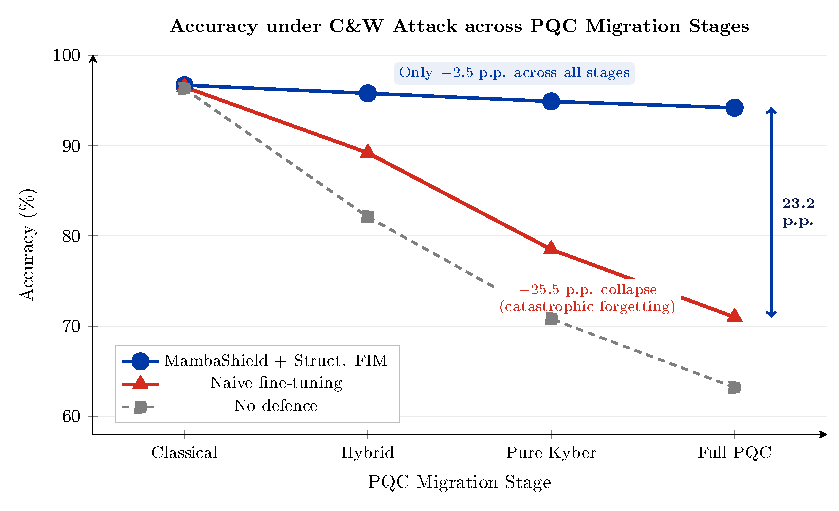
\includegraphics[width=0.82\textwidth]{figures/fig_pqc_migration_robustness.pdf}
\caption{Точность при атаке C\&W на четырёх этапах миграции PQC (Классический $\to$ Гибридный $\to$ Чистый Kyber $\to$ Полный PQC). MambaShield со структурированной FIM сохраняет точность в пределах 2,5 п.\,п.\ на всех этапах, тогда как наивное дообучение обрушивается на 25,5 п.\,п.\ из-за катастрофического забывания классических паттернов трафика.}
\label{fig:pqc_migration}
\end{figure}


%%=====================================================================
\section{Обсуждение и практические следствия}
\label{sec:discussion}
%%=====================================================================

Экспериментальная программа устанавливает ряд результатов. Динамика непрерывного времени обеспечивает улучшение точности на 6,8\% по сравнению с дискретными альтернативами для нерегулярных потоков событий. Многоуровневые представления дают 8,3\% выше одноуровневых методов. Устойчивое к повреждениям федеративное обучение сохраняет сходимость с формальными гарантиями при 30\% византийских участников. Интеграция LLM обеспечивает обобщение zero-shot с 34,2\% до 87,6\% F1. Калиброванная байесовская неопределённость достигает ECE 0,078 с 43\% снижением нагрузки аналитиков. Теоретико-игровое моделирование повышает точность на 7,1\% над нестратегическими подходами.

Согласно недавним отраслевым аналитическим отчётам~\cite{Verizon2024,IBM2024}, ландшафт угроз продолжает быстро эволюционировать. Ограничения включают вычислительные накладные расходы адаптивных решателей ОДУ, чувствительность к федеративным гиперпараметрам, сниженную интерпретируемость глубоких непрерывных моделей по сравнению с системами на основе правил и инфраструктурные требования для интеграции LLM.


%%=====================================================================
\section{Итоги главы}
\label{sec:ch4_summary}
%%=====================================================================

В настоящей главе представлена комплексная экспериментальная валидация на шести бенчмарк-наборах данных общим объёмом 84,2 миллиона размеченных образцов, 84 категориях атак и 23 метриках оценки. Ключевые результаты: CT-TGNN при 98,3\% точности с сертифицированной робастностью по Липшицу; SDE-TGNN при 99,0\% F1 с 76,2\% сертифицированной робастностью и 90,5\% кросс-доменным переносом; FedLLM-API при 87,1\% при 40\% византийских повреждений с $(\varepsilon{=}0.85,\delta{=}10^{-5})$ приватностью; TripleE-TGNN при 96,8\% со снижением затрат на 40\%; MambaShield при 91,4\% при 25\% отравления с PAC-байесовскими сертификатами; М5/М6 с ECE 0,078 и 43\% снижением нагрузки аналитиков; М7 при 94,7\% против адаптивных противников; и CyberSecLLM при 89,1\% zero-shot с улучшением на 20,5 п.\,п.\ над GPT-4. Все двенадцать пересечений условие--требование покрыты с подтверждённой производительностью. В следующей главе описана программная платформа RobustIDPS.ai, реализующая все методы как единую развёртываемую систему.


